\chapter{System Design}
\thispagestyle{plain}
\label{System Design}


\section{Architecture Overview}

The architecture of the system comprises of several modules that process a given input log file. After going through the several components we give out a RDF (Resource Description Framework) file as output. The modular nature of the architecture allows us to add more specialists to the existing framework. Thus, the framework was designed keeping scalability in mind. Figure~\ref{fig:system_architecture} shows the block diagram of the system architecture. It begins with \textit{Tabulate} module, where the input log file is parsed to detect its structure. Once the structure is detected the structured log file is separated into columns. These columns are they passed to the \textit{Decode} stage. In the \textit{Decode} module the columns are checked against various classifiers to find a match. After checking against different classifiers, the columns are given a score against every classifier in the system. The scores form a ranked list of probable classes for the columns in the log file. This ranked list is used in the \textit{Relationship Generator} to identify the relations between various columns in the log file. Once the columns are identified and the relationships have been detected, the \textit{Generate RDF} module will produce a set of RDF triples to represent the inferred semantics. The four major modules have been described in detail in rest of the section.


\begin{figure}[h]
	\centering
	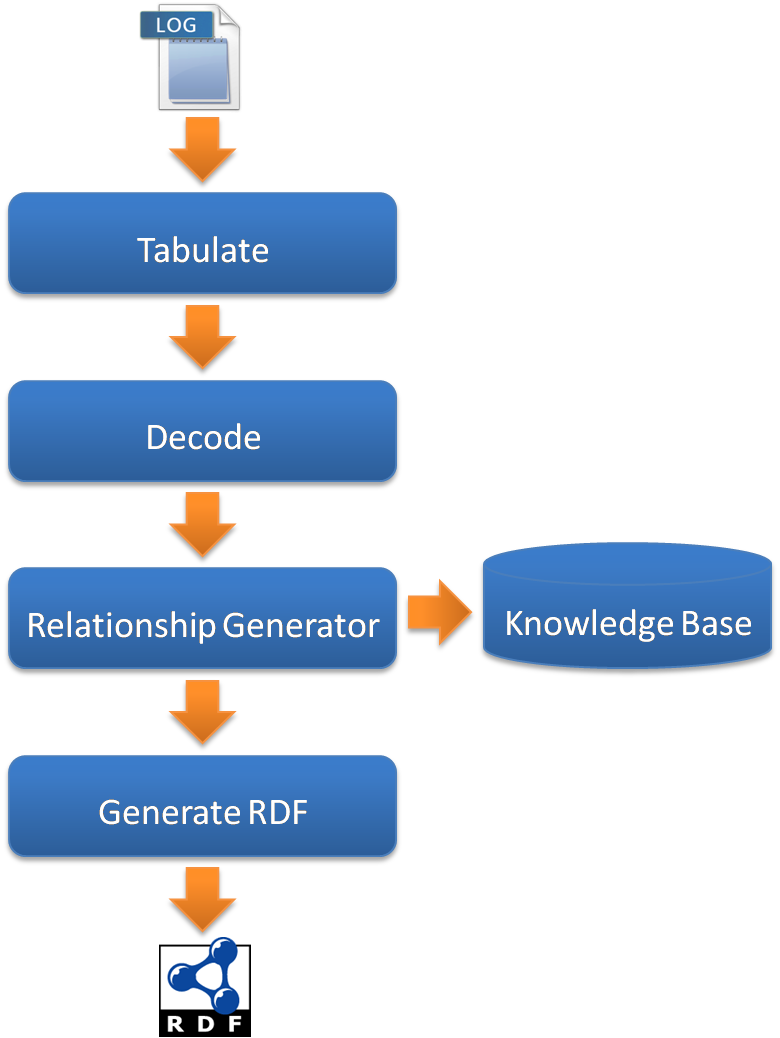
\includegraphics[width=\textwidth, height=0.5\textheight, keepaspectratio] {system_architecture.png}
	\caption{System Architecture}
	\label{fig:system_architecture}
\end{figure}


\subsection{Tabulate}
\label{Tabulate}

The \textit{Tabulate} module takes the structured log file as input and gives out a possible set of columns to the \textit{Decode} module for classification. The input log file can have any structure and the module will try to detect columns in it. The log file undergoes multiple iterations for the following reasons:
\begin{itemize}
\item To split the log file based on delimiters
\item To detect consistent number of columns throughout the log file
\item To detect and separate sub-columns
\end{itemize}

In the first iteration of the \textit{Tabulate} module, we split the log files using generic delimiters like space, square braces, round braces, single and double quotes. For braces and quotes we consider only those that are in pairs. Every row is thus separated in varied number of columns that may or may not be consistent. 

Although most of the lines in a structured log file have fixed number of columns, it is not necessary that after separating on the above delimiters we will get equal number of columns. Also, some log entries can be outliers due to consistency in the way the logs are generated. But in most of the cases, there is a textual description at the end of the log entry which does not have a fixed number of words. If the description is not enclosed in a brace or quote, then it will be divided into several different columns. Considering this fact, we dynamically decide the number of columns that are to be extracted. For this, we put a threshold on the percentage of rows that will be considered in the system. We select rows starting with the ones that have the highest number of columns. We then select the next set of rows that have the second highest number of columns. We continue this process till we reach the threshold number of rows. At this moment we record the number of columns of the current set of rows. This is the number of columns that we choose to output from the system. All the rows having columns less than the selected number of columns are discarded. We keep the threshold pretty high (above 70 \%), so as to collect more number of rows. We also tried keeping the rows that have columns less than the selected number of columns and utilize them in the \textit{Decode} module. It was observed if a large percent of log entries have consistent columns, then the remaining smaller percent usually forms abnormal entries. Thus they create noise in the \textit{Decode} module when trying to detect the class of the column.

In the third iteration, we loop through the columns that are already separated in the previous iterations. In the iteration we check the columns to detect sub-columns. We use the same set of delimiters to split the columns further. If all the elements in a particular columns are separable, then we split the column into multiple sub-columns. Before separation, we run that whole column to check if the whole columns matches any of the known classes. If there is a match found, then there is no need of splitting the column, as we can use the column as a whole.


\subsection{Decode}
\label{Decode}

\subsection{Relationship Generator}
\label{Relationship Generator}

\subsection{Generate RDF}
\label{Generate RDF}


%\subsection{Data Reader}
%\label{Data Reader}
%This module can read data from a local disk or over a network. This module traverse all directories of malware families one by one and grabs the malware sample (.apk file) from that directory for analysis. Each apk file is provided to 'House Keeping' module.
%\subsection{House Keeping}
%\label{House Keeping}
%This module is responsible for installation of malicious application on a android phone. We can use android emulator as well. Following activities are performed by House Keeping module.
%\begin{itemize}
%\item Installation of malicious application on a android phone.
%\item Informing Action Generator module about newly installed application.
%\item Removal of malicious application from a android phone.
%\item Collect log files generated for given application run.
%\end{itemize}
%\subsection{Action Generator}
%\label{Action Generator}
%This module is built on top of 'Android Monkey' tool. As per user configuration, this module generates pseudo-random streams of user events such as clicks, touches or gestures, as well as a number of system-level events. If required user can generate same sequence of actions. As a default action, tool is configured to generate random actions to mimic the user behavior.
%\subsection{Activity Logger}
%\label{Activity Logger}
%This module is responsible for logging all system calls and resource consumption related information on a android phone. This module requires "root" permission and needs to be installed on the "system" partition of the android phone.
%\subsection{Data Preprocessor}
%\label{Data Preprocessor}
%Once all log files are collected for the experiment run, this module converts collected data into single csv formatted file. Two csv file are generated by this module. These files are used for:
%\begin{itemize}
%\item Binary classification, where target is set to binary value (0 or 1).
%\item Multiclass classification, where target is set to "malware family" name.
%\end{itemize}
%\label{Knowledge Generation}
%This module is responsible for data massaging, feature selection and running various algorithms for experiment. This module can be located on local system or in the cloud.

\section{System Input}
\label{System Input}
The system requires android malware repository location. Expected directory structure is shown in figure ~\ref{fig:malware_dir_struct} where every subdirectory represents \(Malware Famliy Name\) and each \(.apk\) file represent the android application specimen. System also expects non malicious application to be placed under \(benign\_apps\) subdirectory.

\begin{figure}[h]
\centering
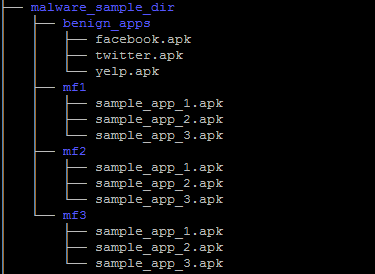
\includegraphics[width=\textwidth, height=0.4\textheight, keepaspectratio]{malware_dir_struct.png}
\caption{Input Directory Structure}
\label{fig:malware_dir_struct}
\end{figure}

\section{System Output}
\label{System Output}
For each malware sample system generates a log file on a Android device. System pulls this log file and places into the same subdirectory from where the application specimen, apk file, was selected for installation. To resolve multiple runs of same application, system adds timestamps at the end of filename. All these logs files are then parsed into a csv file where frequency of each system call forms the feature and malware family name forms the target label. The system generates two out files.
\begin{itemize}
\item b\_android\_apps\_run.csv : file for binary class classification (malicious\/benign).
\item m\_android\_apps\_run.csv : file for multi class classification (malware families).
\end{itemize}
Typically user needs to normalise the input before building a classifier on this data. We perform this step in two stages. 
\begin{itemize}
\item Feature Selection: We use $sparseLDA$ normalization algorithm for feature selection.
\item Normalize: We use Zscore normalization technique for our analysis.
\end{itemize}

This would generate a matrix of size \(N \times W\), where \(W\) is selected features with target as a last column and \(N\) is the number of application run for given dataset. This matrix contains normalized values and then used as a input to various classifiers. Binary classification is done to detect malicious vs benign apps from given data set. Multiclass classification is done to classify given application into malware families. We use various algorithms such as RandomeForest, AdaBoost, SVM, Neural Network, SdA for classification. Results are discussed in the section~\ref{Results}.
